\documentclass{bioinfo}
\usepackage{appendix}
% \usepackage{hyperref}
\copyrightyear{2010}
\pubyear{2010}

\begin{document}
\firstpage{1}
\newcommand{\todo}[1]{\textcolor{red}{#1}}
\newcommand{\update}[1]{\textcolor{blue}{#1}}
\newenvironment{remark}[1][Remark]{\begin{trivlist}
\item[\hskip \labelsep {\bfseries #1}]}{\end{trivlist}}
\title[NETGEM]{NET GEM: Network Embedded analysis of Temporal Gene Expression using Mixtures}
%\title[short Title]{Analysis of temporal gene expression using mixture models}
\author[Sample \textit{et~al}]{Vinay Jethava\,$^{1}$, Torbjorn Karfunkel$^{2}$, Chiranjib Bhattacharyya\,$^{1}$, Devdatt Dubhashi$^{2}$,Goutham N.
  Vemuri$^{3}$\footnote{to whom correspondence should be addressed}}
\address{$^{1}$Computer Science and Automation Department, Indian Institute of Science,
Bangalore, INDIA\\
$^{2}$Department of Computer Science, Chalmers University of
  Technology, G\"oteborg, SWEDEN\\
$^{3}$Systems Biology, Department of Chemical and Biological Engineering, Chalmers University of
Technology, G\"oteborg, SWEDEN\\
}

\history{Received on XXXXX; revised on XXXXX; accepted on XXXXX}

\editor{Associate Editor: XXXXXXX}

\maketitle

\begin{abstract}
\section{Motivation}
Microarrays have become a routine tool in biological enquiry, geared
to measure global gene expression in response to genetic or
environmental perturbations. The outcome is a vast amount of data, for
which many statistical methods have been developed. These methods
identify condition-dependent transcriptional regulation, but are not
suited to analyze time-series data. Furthermore, these methods ignore
the effect of the underlying interaction network of genes or
proteins. Substantial amount of additional information on the
interaction dynamics could be obtained if time were to be treated
appropriately in the context of the interaction network. 

\section{Results}
We present NET GEM, an algorithm that models temporal gene expression
data using Hidden Markov Models, within the constraints of an
underlying network. We used NET GEM to identify the dynamics of
interactions in wild-type Saccharomyces cerevisiae or its isogenic
mutant during continuously changing nutritional environment. NET GEM
identified significant changes in the interactions between
\textcolor{red}{[to be filled]} 

\section{Availability:}
The source code for NET GEMM is available from http://www.website
\textcolor{red}{[will fill in before submission. The website mentions
  having a permanent website. I propose http://129.16.106.142/ where
  we collect all the tools. We should include a readme.txt that should
  have info on input files needed, their formatting, choosing
  parameters, output file description and their interpretation]} 

\section{Contact:} goutham@chalmers.se %\href{goutham@chalmers.se}{goutham@chalmers.se}
\end{abstract}

\section{Introduction}
%To be filled. Ideas - strains, time important, relate to KELLER VERY GENTLY!
%focus on special techniques.

Microarrays have become a routine tool in the biological inquiry of
transcriptional regulation. Gene expression microarrays present a
snapshot of the transcriptional profile of all the genes at the time
of measurement, resulting in a vast amount of data. Current methods to
analyze the data are geared to identify genes that have differential
expression in response to genetic or environmental perturbations
\textcolor{red}{[REFS]}. There are numerous statistical methods to
cluster genes, and all of them have been enjoyed varying degree of
success in discovering new mechanisms of transcriptional
regulation. \textcolor{red}{[(Torbjorn needs to write brief intro to
  the different methods to cluster genes and theor drawbacks, keeping
  in mind this is not a review of the methods. I can think of PCA,
  k-means, Self Organized Maps, supervised learning methods such as
  Support Vector Machines, anything else I missed. All this needs to
  be less than 100 words]}  All these methods have been able to
identify the condition-specific gene expression and map the
transcription regulatory network by identifying binding sites of the
promoters \textcolor{red}{[REFS]}. The general idea of all these
methods is to cluster genes that have similar expression profile,
based on the assumption that co-expressed genes are likely to be
co-regulated. 
An inherent drawback with the presently available methods is that they
are not well suited to analyze temporal gene expression data. Time
course data on gene expression provides substantial insight into the
dynamics of transcriptional regulation, such as sequential events in
invoking transcriptional response, any time lag in the process and
relate the amplitude of the signal to different perturbations
\textcolor{red}{[general REF on time series]}. Since time series data
have a natural temporal ordering, using conventional methods to
analyze time series data will fail to capture the internal structure
of the data. Moreover, these methods also fail to consider that
observations closer in time are likely to be closer than temporally
distant observations\textcolor{red}{[ - this is why it is important to
  include timepoints into the analysis]}. Unfortunately, the
traditional framework of time series analysis cannot be used to
analyze temporal gene expression data due to the small number of
observations (time points), owing to cost and/or biological
limitations. Recognizing these drawbacks, there has been a growing
interest to develop dedicated algorithms that address these drawbacks
\textcolor{red}{[REFS]}.  
\textcolor{red}{[Torbjorn to review (less than 100 words) EDGE, STEM,
  KELLER, TARM, and others that I included in another document. This
  can also go into the intro of Manuscript 3]} 

Hidden markov models (HMMs) capture the one-way ordering of time such
that observations at any time point are dependent on the previous
values \textcolor{red}{[REFS]}. HMMs were used to analyze temporal
gene expression data  
\textcolor{red}{[Vinay to review (less than 50 words) previous
  analysis of microarray data using HMM, only some of the references
  are provided]}. These algorithms do not consider the underlying
network topology of regulation. In this article, we present
network-embedded analysis of temporal gene expression using mixture
models (NET GEM). This method takes into account the functional
catogories of the interacting genes during the inference procedure. 

\textcolor{red}{[Vinay to complete the sentence]} 

We applied NET GEM to publicly available time-series gene expression
data in Saccharomyces cerevisiae. The available of a highly curated
interaction network for this organism makes it an ideal platform for
testing the method. We selected two time-series datasets in which the
nutritional environment changed with time, one without any genetic
perturbations and one with a deletion in the SFP1 transcription
factor. The first dataset consists of expression of genes during the
gradual transition from carbon starvation to nitrogen starvation in a
D-stat under aerobic or anaerobic conditions \todo{(Farzadfard et al.,
2010)}. Almost a fourth of the genome underwent transcriptional changes
in response to the transition. The dominant transcription factor that
brought about these changes was Sfp1, which is known to assimilate
signals from the environment and coordinates growth with metabolism
\todo{(Marion et al., 2004)}. The second dataset measures the temporal
changes in gene expression upon sudden exposure of a strain of
S. cerevisiae in which Sfp1 was deleted to glucose \todo{(Cipollina et al.,
2009)}. Using these datasets, NET GEM identified
\textcolor{red}{[dynamics of interactions between genes, functional
  categories, etc  - Vinay to complete the sentence]} 
 
\begin{methods}
\section{Methods}
We describe our approach to the problem of inference of the temporally
evolving interactions in an underlying network.
\subsection{Dataset}
 Temporal gene expression datasets were downloaded from Gene
 Expression Omnibus using accession numbers XXXXX and XXXXX. The two
 datasets were obtained using Affymetrix platform. The first dataset
 contained the expression profiles of the genes in S. cerevisiae
 during the transition from carbon limitation to nitrogen limitation
 under aerobic or anaerobic conditions. The transition was achieved by
 gradual increment of glucose availability in the feed to the cells,
 while keeping the nitrogen concentration constant in a D-stat
 (Farzadfard et al., 2010). Beyond a certain concentration of glucose,
 nitrogen became the limiting nutrient. The cells underwent changes
 related to growth rate as well as metabolism. Analysis of genes whose
 expression significantly changed indicated that Sfp1 transcription
 factor played a dominant role in the bringing out the response to
 transition. In the interest of coherence, we chose a dataset that
 contains the temporal gene expression profiles in sfp1 deletion
 mutant and its isogenic reference at different time points after
 pulsing steadily growing cells with glucose. The data was measured at
 six time points after the pulse. These data were analyzed using
 conventional methods, assuming that all time points are independent.

\subsection{Construction of the interaction network}

The yeast interaction network was constructed using data from
previously published datasets. Interactions between proteins that
occurred in at least two independent datasets were considered. These
interactions were downloaded from
BIND~\cite{Bader:2003:Nucleic-Acids-Res:12519993}, MIPS~\cite{MIPS},
MINT~\cite{citeulike:3733950}, DIP~\cite{citeulike:226627}  and
BioGRID~\cite{citeulike:814974}  and literature data \todo{(5-6
references)}. The construction of this high-confidence network was
described in detail previously \todo{(Musigkain et al., 2010)}. The
transcriptional regulatory network (interactions between transcription
factors and genes) was downloaded directly from
YEASTRACT~\cite{citeulike:473096}. The two networks were combined and
the nature of  interactions was not distinguished for the analysis.


\subsection{Known network}
We assume that the base underlying network of interactions is known as a
graph $G=(V,E)$. Under different conditions, some of the edges are 
switched on or off, or, more generally set at various levels of
activation, $\mathcal W$. Also, the same edge may be active in one
strain and not in others at any given time point. Thus, we model the
state of the network by activation levels, $\mathbf{w}^{s}(t) = \{w^s_{e}(t)\}_{e
\in E}$, where $w^s_{e}(t)$ is the activation level of the edge $e$ at time $t$ in strain $s$. 

We use the notation $x^{s}_{e}(t)$ to denote the expression
levels for genes, $i$ and $j$, consisting the edge, $e=(i,j)\in E$,
for strain, $s$, at time $t$. Similarly,  $x_{e}^{1:S}(t_{a}:t_{b})$
denotes the observations for gene expression levels for edge,
$e=(i,j)$, over the set of strains, $\{1,\ldots, S\}$; for the time
interval, $\{t_{a}, (t_{a}+1), \ldots, t_{b}\}$. 

The observed gene expression levels, $\mathbf{x}^{s}(t)$, for an strain
$s$ at time $t$ are modeled as an Ising system \cite{Song09KELLER}:
\begin{equation}
\label{eq:ising}
 P\left(\mathbf{x}^{s}(t) | \mathbf{w}^{s}(t)\right) = 
      \frac{1}{Z} \exp \left( - \sum_{(i,j) \in E} w^s_{e}(t)
        x^{s}_i(t) x^{s}_j(t)\right)  
\end{equation}
We assume that the weights evolve according to the markov chain, i.e.,
$P(\mathbf{w}^{s}(t+1) = \mathbf{w}_{t+1} |  \mathbf{w}^{s}(t) =
  \mathbf{w}_{t}, \mathbf{w}^{s}(t-1) = \mathbf{w}_{t-1},
  \ldots) = P\left(\mathbf{w}^{s}(t+1) = \mathbf{w}_{t+1} |  \mathbf{w}^{s}(t) =
  \mathbf{w}_{t}\right)$ for each strain. 
% We denote $Q$ as the
% transition probability of strain, $s$, such that
% \begin{equation}
%   \label{eq:Q-s}
%   Q^{s}(l, m) = P(\mathbf{w}^{s}(t+1) = \mathbf{w}_{m} |  \mathbf{w}^{s}(t) =
%   \mathbf{w}_{l})
% \end{equation}
However, the strains in the given problem are just slightly altered
networks where a few genes have been knocked out of the
network. Therefore, most of the network remains the same across
strains with only the ``close'' neighbourhood of the knocked out genes
being affected. Thus, if one looks at a ``far'' edge,
$e_{far}$, the activation strength, $w_{e_{far}}(t)$, should be the
same across strains  the gene expression data for the edge strains,
$x^{1:S}_{e_{far}}(t)$, should be like i.i.d. samples, generated with
the same activation strength, $w_{e_{far}}(t)$. In the following discussion, 
we present a heuristic method which incorporates the ideas mentioned
above into the inference problem. 
\subsubsection{Strain Damping Heuristic } 
We assume that the weights corresponding to the reference strain
$\mathbf{w}(t)$ evolve according to a Markov law given by a matrix $Q$,
where $Q(l, m) = P(\mathbf{w}(t+1) = \mathbf{w}_{m} | {\mathbf w}(t)
= \mathbf{w}_{l})$ with the property that $\sum_{m} Q(l, m) = 1$ for
all the initial states $\mathbf{w}_{l}$. For other strains, we assume
that the corresponding values are just slightly perturbed; thus
\begin{equation}
  \label{eq:damping}
 w^s_e(t) = w_e(t) \Gamma^s_e
\end{equation}
The perturbing parameters $\Gamma^s_e$ are determined
deterministically from the underlying network $G$ by
\begin{equation}
  \label{eq:edge-damping}
\Gamma^s(i,j) = (1 - \gamma^s_i)(1 - \gamma^s_j)  
\end{equation}
where $\gamma^s_i \in [0,1]$ is a label determined by how far the gene
$i$ is in the underlying network to one of the genes knocked out in
strain $s$. We note that the deterministic nature of the damping
implies that all strains evolve similarly, i.e., $Q^{s} = Q\;
\forall \; s$. This allows us to incorporate the information for gene
expression levels in the different strains while learning the temporal
evolution characteristics. 

There is a tradeoff between using more sophisticated conditional
probability models $p(\mathbf{w}^{s}(t) |\mathbf{w}^{0}(t))$ involving more
parameters to be learnt and the limited amount of experimental
data.\todo{EXPAND FURTHER?} 

We compute the damping factor, $\gamma^s_i$, for the genes
as follows: If the gene, $i$, is knocked out in strain $s$, then we
label it as $\gamma^s_i=0$. Now, we diffuse the labels across the
graph  such that $\gamma^{s}_i = \frac{1}{d(i)} \beta
\sum_{j\in N(i)} \gamma_j^s$, i.e., the damping factor at a node is
the average of the damping factors at its neighbours.    

 Intutitively, while $\Gamma_e = 0$ for an edge 
directly incident to one of the knocked out genes, the perturbation
gradually damps out with distance from the knocked out gene and for
an edge $e$ far away from one of the knocked out genes, $\Gamma_e
\approx 1$.

Thus, the problem is a simple HMM~\cite{Rabiner89hmm} with
$\mathbf{x}^{1:S}(t)$ and $\mathbf{w}(t)$ as the observation and  the
hidden variable at time $t$, and $Q=P(\mathbf{w}(t+1)| \mathbf{w}(t))$
the unknown parameter to be learnt. 
We note that an application of the standard forward-backward algorithm
to compute the probability distribution over the weight states
requires $O({\mathcal W}^{N_{e}}T)$ computations, where, ${\mathcal
  W}$ is the number of possible discrete states for an edge activation
strength, $N_{e}$ is the total number of edges, and $T$ is the time
period for which observations are made.  This is prohibitively
expensive and in the following section, we outline an approximation to
solve this problem.

% The updates,  $q_{k}^{(n+1)}(w, w')$, in \eqref{eq:cluster_update} provide a likelihood
% estimate, which can be used to compute the parameters, $\Theta_{k}$, 
% for the posterior distribution of the transition probability matrix, $Q_{k}$, as follows: 
% \begin{eqnarray}
%   \label{eq:q_posterior}
%   \theta_{k}^{(n+1)}(i, j) &=&  \theta_{k}^{(n+1)}(i, j) +
%   q_{k}^{(n+1)}(i, j )
% \end{eqnarray}
% Now we proceed to outline the procedure to infer the unknown parameters in
% the model. We employ the standard Expectation Maximization (EM) technique for MAP
% learning~\cite{Beal03,Dempster77em} which gives the estimate as, 
% \begin{equation}
%   \label{eq:q_em_map}
%   \begin{array}[h]{llll}
%   \textrm{E-step:} & {\mathcal L}(Q; Q^{(n)}) &=&  E_{W^{|}}  [ \ln
%   P(\mathbf{x}^{1:S}(1:T), \mathbf{w}(1:T) | Q)] \\ 
% &&&\nonumber\\
% \textrm{where} & P(W^{|}) &\equiv & P({\mathbf{w}(1:T)| \mathbf{x}^{1:S}(1:T),
%   Q^{(n)}}) \nonumber \\
% &&&\nonumber\\
%   \textrm{M-step:} & \hat{Q}_{MAP} &=& \arg\max_{Q} (\ln P(Q) +
%   {\mathcal L}(Q; Q^{(n)} ) ) \\
%   \end{array}
% \end{equation}
% where $\mathbf{w}(1:T)$ is the hidden variable denoting the
% activation strengths $\{w_{e}(t)\}$ over all edges $e\in E$ and times
% $t=1,\ldots,T$ are the hidden variables. The conditional probability,
% $P(\mathbf{w}({1:T})| \mathbf{x}^{1:S}(1:T), Q^{(n)})$, in the  likelihood term, $ {\mathcal L}(Q; Q^{(n)} )$, can be computed by the forward-backward algorithms~\cite{Rabiner89hmm}.
% We apply the standard Expectation
%where $ {\mathcal L}(Q; Q^{(n)} )$ is the likelihood function given by
% and the forward-backward algorithm. 
% This computation is prohibitively expensive for moderate sized networks. 
\subsubsection{Factorial approximation}
As noted in the previous section, applying the standard forward
backward algorithm is prohibitively expensive for moderate sized
graphs. So, we make the simplifying assumption that the weights are
evolving \emph{independent} of each other. This leads to the factorial
approximation~\cite{DBLP:journals/ml/GhahramaniJ97,Mclachlan97embook} for weight distribution, i.e.,  
\begin{eqnarray}
  \label{eq:q_mf}
  \hat{P}({\mathbf w}^{t}) &=& \prod_{e\in E} P_{e}(w_{e}^{t}) \\
  \hat{P}(w_{e}^{t+1} = w_{l} | w_{e}^{t} = w_{m}) &=& q_{e}(l, m)
\end{eqnarray}
Now, the parameter to be learnt is the transition matrix $Q_{e}$ for
each edge, $e = (i, j) \in E$.  We solve the Expectation
Maximization~(EM)\cite{Dempster77em} for MAP problem for each edge,
$e$,\footnote{The quality of the factorial approximation is discussed in the appendix} 
\begin{equation}
  \label{eq:q-edge_em_map}
  \begin{array}[h]{llll}
  \textrm{E-step:} & {\mathcal L}(Q_{e}; Q_{e}^{(n)}) &=&
  E_{w_{e}^{|} }  [ \ln P(\mathbf{x}_{e}^{1:S}(1:T),
  \mathbf{w}_{e}({1:T}) | Q_{e})] \\
\vspace{2 mm}
  \textrm{M-step:} & \hat{Q}_{e}^{(n+1)} &=& \arg\max_{Q_{e}} (\ln P(Q_{e}) +
  {\mathcal L}(Q_{e}; Q_{e}^{(n)} ) ) 
  \end{array}
\end{equation}
where $W^{|}_{e}$ is the conditioned variable, $w_{e}(1:T)|
\mathbf{x}_{e}^{1:S}(1:T), Q_{e}^{(n)}$ and $Q_{e}^{(n)}$ is the
MAP estimate for the transition probability, $Q_{e}$, at the $n^{th}$
iteration of the algorithm. 
We assume that the data for strain, $s$, is independently generated
based on the Ising model in (\ref{eq:ising}) with the weights that are
damped versions (\ref{eq:damping}) of the weights in the original 
strain. This leads to the observation model specified as:
\begin{eqnarray}
  \label{eq:obs}
  o^{t}_{e}(l) &=& P(x_{e}^{1:S}(t) | w_{e}(t) = w_{l}) \\
\label{eq:obs2}
& = & \frac{1}{Z} \prod_{s=1}^{S} P(x_{e}^{s}(t) | w_{e}(t) = w_{l})
\\
\label{eq:obs3}
& = & \frac{\exp\left\{ - w_{l}\big(\sum_{s=1}^{S}
      x^{s}_{i}(t)x^{s}_{j}(t) \Gamma^{s}(i,j)\big)
  \right\}}{\sum^{\mathcal W}_{l=1}\exp\left\{ - w_{l}\big(\sum_{s=1}^{S}  x^{s}_{i}(t)x^{s}_{j}(t) \Gamma^{s}(i,j)\big) \right\}}
\end{eqnarray}
The update equations for computing the forward and backward
probability distributions are given as:
\begin{eqnarray}
  \label{eq:update}
  f^{t+1}_{e}(m) &=& P(x_{e}^{1:S}(1:t) , w_{e}(t+1) = w_{m} | Q^{(n)}_{e}) \\
&=& o^{t+1}_{e}(m) \sum_{l=1}^{{\mathcal W}} f_{e}^{t}(l) q_{e}^{(n)}(l, m) \\
  b^{t}_{e}(l) &=& P(x^{1:S}_{e}((t+1):T) | w_{e}(t) = w_{l},
  Q^{(n)}_{e})  \\
\label{eq:update-1}
&=& \sum_{m=1}^{{\mathcal W}} q_{e}^{(n)}(l, m) o^{t+1}_{e}(m) b^{t+1}_{e}(m)
\end{eqnarray}
and the joint probability as
\begin{eqnarray}
  \label{eq:p-joint}
  \xi_{e}^{t}(l,m) &=& P(w_{e}(t,t+1) =(w_{l}, w_{m}) |
  x^{1:S}_{e}(1:T), Q^{(n)}_{e}) \\
&\propto& f_{e}^{t}(l) q_{e}^{(n)}(l, m) o_{e}^{t+1}(m) b^{t+1}(m) 
\end{eqnarray}

Often, there is domain knowledge available which can be incorporated
in the form of prior distribution. For example, one may know that most
of the edges are inactive about 50\% of the time.

% [ALTERNATIVE VIEW IN TERMS OF KL DIVERGENCE]

\subsubsection{Dirichlet prior}
We model the transition probabilities matrices as dirichlet distributions,
such that  the prior on the transition probabilities matrix, $Q$, 
given the parameter, $\Theta$, is
\begin{eqnarray}
  \label{eq:q_prior}
  P(\vec{q}_{l} | \vec{\theta}_{l}) &\sim& Dir(q_{l1}, \ldots, q_{l\mathcal{W}} ;
  \theta_{l1},\ldots, \theta_{l\mathcal{W}}) \\
&=& \frac{1}{B(\vec{\theta}_{l})} \prod_{m=1}^{\mathcal{W}} q_{lm}^{\theta_{lm}-1}
\end{eqnarray}
where $\vec{\theta}_{l}=[\theta_{l1},\ldots,\theta_{l\mathcal{W}}]$ and
$B(\vec{\theta}_{l})$ is the multinomial beta
function~\cite{Gelman03bayesian}.

This leads to the update equation for the MAP estimate for transition
probabilities, $q(l,m)$, obtained by the maximization step in (\ref{eq:q-edge_em_map}) as
\begin{equation}
  \label{eq:q-update}
  q^{(n+1)}_{e}(l, m) = \frac{(\theta_{lm}-1) + \sum_{t=1}^{T-1} \xi^{t}_{e}(l,
    m) }{\sum_{m} (\theta_{lm} -1) + \sum^{T-1}_{t=1} \sum^{\mathcal
      W}_{m=1} \xi^{t}_{e}(l,m)}
\end{equation}
\subsubsection{Cluster Similarity: } 
We can often group the network interactions into categories  based on
domain knowledge about the functional classification of genes.  For
example, one might model the genes that participate in sugar
metabolism as one 
component, while treating genes involved in DNA synthesis as another
component.  This allows us a
simplification that we need to  consider only evolution over the
\emph{components}(or \emph{clusters}), $A_k$ of edges,  which are parameterized by the
cluster transition, $Q_{k}$ for  cluster $A_k$. 

Then, the update equations for the transition probability matrix,
$Q_k$, for the cluster, $A_k$ are as follows,
\begin{eqnarray}
  \label{eq:cluster_update}
  q_{k}^{(n+1)}(l, m)   &=& \frac{(\theta^{(k)}_{lm} -1) + \sum_{e \in A_k} \sum_{t=1}^{T-1} \xi^{t}_{e}(l,m)}{ (\theta^{(k)}_{ij} -1) + \sum_{e \in A_k} \sum_{t=1}^{T-1}
   \sum_{m} \xi^{t}_{e}(l,m)} \nonumber \\
\end{eqnarray}
where $\theta^{(k)}$ is the dirichlet parameter matrix for cluster,
$A_{k}$.
\begin{figure}[h]
  \centering
  \fbox{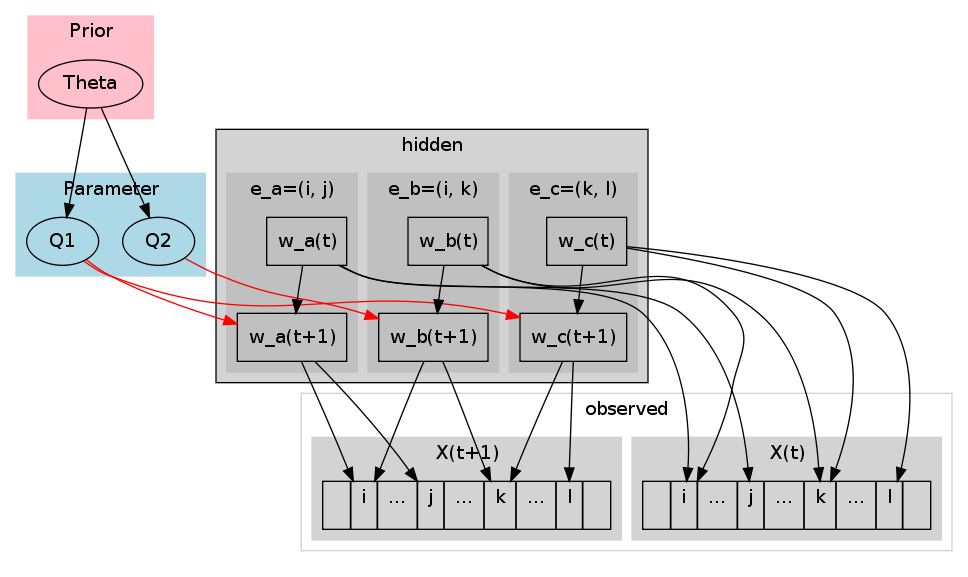
\includegraphics[scale=0.23]{images/factorial2}}
  \caption{Single functional classification model. Here, the
    edges $a, \,c$ belong to evolution class $1$, while edge $b$
    belongs to evolution class $2$. $X_{t}$ is the observed gene
    expression level at time $t$; $w_{e}(t)$ is the hidden variable
    denoting interaction strength for edge $e$ at time $t$; $Q_{i}$
    are the evolution characteristic for class $i$; and $\theta$ is
    the prior based on domain knowledge.}
  \label{fig:factorial}
\end{figure}


Figure~\ref{fig:factorial} shows the graphical model corresponding to
the known network model with cluster similarity. We present an
extension of the current model to handle multiple functional
categories for genes.
 
\subsection{Mixture Model}
\label{sec:mixture-model}
% Significant progress has been
% made towards identifying the functional roles of the genes, resulting
% in a heirarchical classification of genomes based on their functional
% roles~\cite{DBLP:journals/nar/MewesAHLP97}. 
\update{This section presents our approach to incorporating the
  functional categories of genes in our analysis. Since, genes belong
  to multiple categories, a mixture model is a naturally suited model
  to handle the influence of multiple functional categories in the
  inference procedure. 
%We seek to incorporate
%this information in our inference algorithm. \textcolor{red}{EXPAND ON GENE CLUSTER}
This allows us to explore  the relationship between functional
categories and the temporal evolution characteristics of the genes
which fall in the same functional category.
}
We now define the problem concretely. There are $H$ possible gene
categories. Each gene can be a member of one or more hierarchical
classes, $\mathcal{C}=\{C_{1},\ldots , C_{H}\}$, where the
hierarchical class $C_{h}$ is characterized by evolution matrix,
$Q_{h}$. The evolution probability matrix, $Q_{e}$, for each edge,
$e\in E$, is given as 
\begin{equation}
  \label{eq:q-mixture}
  Q_{e} = \sum_{h=1}^{H} \alpha_{e,h} Q_{h}
\end{equation}
where $\alpha_{e,h}$ denotes the influence of hierarchical class
$C_{h}$ in the edge, $e$, such that $\sum_{h} \alpha_{e, h} = 1$
for all edges $e \in E$. We define the random variable
$\mathbf{y}^{1:T} = \{y_e^t\}$ for all edges, $e \in E$,  and times,
$t=\{1,\ldots, T\}$ where $y^t_e$
denotes the component from which the evolution characteristics are
chosen at time $t$ for edge $e$ such that the event $y_e^t = h$
implies that $P(w_e^{t+1}= w_m | w^t_e =w_l, y_e^t = h) = q_h(l, m)$.
% Let $\gamma_e^t(h)$ be the probability $P(y^t_e =h )$.

We now outline the expectation maximization procedure~\cite{Bilmes98agentle,Mclachlan97embook} which
iteratively learns the unknown quantity, $\Psi = \{Q_{h},
\alpha_{e,h}\}$, for $h \in {\mathcal H} = \{1,\ldots, H\}$ and $e \in
E$ where  $Q_{h}$ is the class evolution
probability matrix for class, $C_h$, and $\alpha_{e,h}$ is the mixing
proportion for  edge, $e$ and class $C_h$; and $\Omega =
\{\mathbf{y}^{1:T},\mathbf{w}^{1:T}\}$ is
the hidden variable.  Let $\Psi^{(n)} = \{\alpha^{(n)}_{e,h},
Q^{(n)}_h\}$ be the estimates at the $n^{th}$ iteration. Then, 
\begin{equation}
  \label{eq:q-edge-mixture-em}
  \begin{array}[h]{llll}
  \textrm{E-step:} & {\mathcal L}(\Psi; \Psi^{(n)}) &=&
  E_{\Omega^{|} }  [ \ln P(\mathbf{x}^{1:S}(1:T), \Omega({1:T}) | \Psi({1:T}))] \\
\vspace{2 mm}
  \textrm{M-step:} & \hat{\Psi}^{(n+1)} &=& \arg\max_{\Psi} (\ln P(\Psi) +
  {\mathcal L}(\Psi; \Psi^{(n)} ) ) 
  \end{array}
\end{equation}
where $\Omega^{|}$ is the conditioned variable $(\mathbf{w}^{1:T},
\mathbf{y}^{1:T} | \mathbf{x}^{1:S}(1:T),  \Psi^{(n)})$.

The factorial approximation in the previous section allows us to
compute the probability distribution over the edges independently.
% The edge evolution matrix, $Q^{(n)}_e$ is given as: 
% \begin{equation}
%   \label{eq:q-e-mixture}
%   q_e^{(n)}(l,m) = \sum_{h=1}^H \alpha^{(n)}_{e,h} Q^{(n)}_h(l,m)
% \end{equation}
% \begin{remark}[VJ: ]
\footnote{Part of this section may be moved to appendix.}
% \end{remark}
The observation model, $o^t_e(l)=P(x^{1:S}_e(t) | w^t_e=w_l)$ , remains unchanged as in
(\ref{eq:obs})-(\ref{eq:obs3}). 
%The forward iterates, $f_e^{t}(m)$, and the backward iterates,
%$b^t_e(m)$, remain unchanged as in (\ref{eq:update})-(\ref{eq:update-1}). 
The forward iterates, $f_e^t(l, h)$ and backward iterates, $b_e^t(l,
h)$ can  be computed as follows: 
\begin{eqnarray}
  \label{eq:mixture-update}
  f^{t}_{e}(m, h) &=& P(x_{e}^{1:S}(1:t) , w_{e}^{t} = w_{m},
  y_e^t = h | \Psi^{(n)}_{e}) \\
&=& P(x^{1:S}_e(t) | w_m) \sum_{w_l} \sum_{h'}
\Big[ P(y^t_e=h | \alpha^{(n)})  \nonumber \\
&\times& P(w_m | w^{t-1}_e = w_l, y^{t-1}_e = h')  \times f_e^{t-1}(l, h')
\Big]\\
%% final forward equation
&=& o^{t}_{e}(m) \sum_{l=1}^{{\mathcal W}} \sum_{h'=1}^H
f_{e}^{t-1}(l, h') \alpha_h^{(n)} q_{h'}^{(n)}(l, m) \\
%% backward equations
  b^{t}_{e}(m, h) &=& P(x^{1:S}_{e}((t+1):T) | w_{e}(t) = w_{m}, y_e^{t}=h,
  \Psi^{(n)}_{e})  \\
&=&  \sum_{w_l} \sum_{h'} \Big[ P(x^{1:S}_e(t+1) | w^{t+1}_e = w_l)
  b_e^{t+1}(l, h')\nonumber \\
&\times& P(w^{t+1}_e = w_l | w_m, y^{t}_e = h)   P(y^{t+1}_e=h' | \alpha^{(n)}) 
\Big]\\
%% final backward equation
\label{eq:mixture-update-1}
&=& \sum_{m=1}^{{\mathcal W}}\sum_{h'=1}^H q_{h}^{(n)}(m, l) o^{t+1}_{e}(l) \alpha^{(n)}_{h'}b^{t+1}_{e}(l,h')
\end{eqnarray}
The conditional probability $P(\Omega_e^{t}=(w_l, h), \Omega_e^{t+1}
=(w_m, h') | \mathbf{x}_e^{1:S}(1:T) , \Psi^{(n)})$ denoted by $\xi^t_e(l,m,h,h') $ can be computed as
\begin{equation}
  \label{eq:mixture-p-cond}
  \xi^t_e(l,m,h,h') \propto f^t_e(l,h)\alpha_{h'}^{(n)} q^{(n)}_h(l,m)
  o^{t+1}_e(m) b_e^{t+1}(m, h')
\end{equation}
The likelihood term, $ {\mathcal L}(\Psi; \Psi^{(n)})$, in (\ref{eq:q-edge-mixture-em}) can be expressed
in terms of the conditioned edge probabilities, $\xi^t_e$, in
(\ref{eq:mixture-p-cond}) as 
\begin{eqnarray}
  \label{eq:mixture-L-edge}
  {\mathcal L}(\Psi; \Psi^{(n)}) &=& \sum_{e\in E}\sum_{t=1}^{T-1}
  \mathbf{E}_{\xi^t_e}[\ln q_h(l, m) + \ln \alpha_{e,h'}]
\end{eqnarray}
subject to the constraints
\begin{eqnarray}
  \label{eq:mixture-q-constraint} \sum_{m} q_h(l,m) &=& 1 \quad\forall h \\
   \label{eq:mixture-alpha-constraint} \sum_{h} \alpha_{e,h} &=& 1 \quad\forall e
\end{eqnarray}
\subsubsection{Domain knowledge:}
We incorporate the effect of the functional classification of
genes on the mixture components,
$\vec{\alpha}_e$, for an edge, $e$, by using a dirichlet prior of the form:
\begin{eqnarray}
  \label{eq:hier-prior}
  P(\vec{\alpha}_e) &\sim& Dir(\alpha_{e,1},\ldots, \alpha_{e,H};
  \gamma_{e,1},\ldots, \gamma_{e,H}) 
\end{eqnarray}
with the prior parameter, $\gamma_{e,h}$, for the edge, $e=(i,j)$, of the
form 
\begin{equation}
  \label{eq:mixture-prior}
  \gamma_{e,h} = \Big\{ \begin{array}{ll}
                       \gamma_p & \textrm{if genes }  i \textrm{ or } j
                       \textrm{ in class } h \\
                       \gamma_o & \textrm{otherwise}
                       \end{array}
\end{equation}
The maximization step in (\ref{eq:q-edge-mixture-em}) can  be done
separately for $q_h(l,m)$ and $\alpha_{e,h'}$ independently. We use
the priors in (\ref{eq:q_prior}) and
(\ref{eq:hier-prior})-(\ref{eq:mixture-prior}), and the constraints in
(\ref{eq:mixture-q-constraint})-(\ref{eq:mixture-alpha-constraint}) to
obtain the following update equations:%\footnote{\textcolor{red}{can be expanded lagrangian partial derivative}}
\begin{eqnarray}
  \label{eq:mixture-alpha-update}
  \alpha_{e,h'}^{(n+1)} =&  \frac{(\gamma_{e,h'}-1) + \sum_{t=1}^{T-1} \sum_{l,m,h}\xi^{t}_{e}(l,
    m,h,h') }{\sum_{h'} (\gamma_{e,h'} -1) + \sum^{T-1}_{t=1}
    \sum_{l,m,h,h'} \xi^{t}_{e}(l,m,h,h')} & \\
\label{eq:mixture-q-update} 
q^{(n+1)}_h(l,m) =&  \frac{(\theta_{lm}-1) + \sum_e \sum_{t=1}^{T-1}\sum_{h'}\xi^{t}_{e}(l,
    m,h,h') }{\sum_{m} (\theta_{lm} -1) + \sum_e \sum^{T-1}_{t=1}
    \sum_{m,h'} \xi^{t}_{e}(l,m,h,h')} &
\end{eqnarray}

% The expectation step requires computation of the likelihood term
% ${\mathcal L}(\Psi;\Psi^{(n)})$ which involves expectation over terms
% $\log (\sum_h \alpha_{e,h}q_{h}(l, m) )$. Following standard mixture
% model techniques~\cite{Bilmes98agentle},
% \begin{equation}
%   \label{eq:em-mixture-exp1}
%    A
% \end{equation}

% We define a random variable, $Y^t_e(l,m)$, such that if $Y^t_e(l,m) = h$
% then the probability $P(w^{t+1}_e = w_m | w^{t}_e = w_l) = q_h(l,
% m)$, i.e., the $h^{th}$ mixing component is active. Let
% $\beta^{t}_{e,h}(l,m)$ denote the probability of the event $Y^t_e(l,m)
% = h$, i.e., $\beta^{t}_{e,h}(l,m)=P(Y^t_e(l,m)= h)$ and $\sum_h
% \beta^t_{e,h}(l,m)=1$.

% \subsection{Model 2: Regularization for unknown network}
% % We consider the exponential random graph model proposed by 

% We use the laplacian prior for the weights as follows $P(w) =\frac{\beta}{2} \exp(-\beta
% ||w||_{1})$. We 
\end{methods}
\section{Experiments}
We present the experiments performed on synthetic and actual datasets
in this section. We compare the factorial weights and the mixture
model against a standard implementation of HMM which learn
the evolution characteristic for the system jointly in
\ref{sec:validation} and present the results on a synthetic dataset in \ref{sec:synthetic-dataset}.

\subsection{\update{Validation}}
\label{sec:validation}
We choose a synthetic graph with $N=5$ nodes (genes) and $H=10$ functional
classes. The genes are randomly assigned classes  such that each
node is a member of $N_{av}=1.5$ classes on average. The weights take
possible values in $\{-1, 1\}$, and the evolution characteristic, $Q_{e}$ for
each weight is a mixture based on the interacting genes.  We compare our methods to
estimate the overall transition probability matrix, $Q_{large}$, with
the results obtained from an standard implementation of 
HMM\footnote{http://people.cs.ubc.ca/~murphyk/Software/HMM/hmm.html}
for $N=20$ random trials. 

Figure~\ref{fig:validation-t} shows the comparison between different
methods with increasing length of the sequence, $T$. We note that the
standard HMM requires longer sequences to get comparable results with
factorial and mixture model approach. Figure~\ref{fig:validation-s} compares the
methods with increasing number of strains present (with at most 1 gene
knocked out). We note that the performance of the factorial weights
assumption shows a slight improvement with increasing number of
strains. 
\begin{figure}[h]
  \centering
  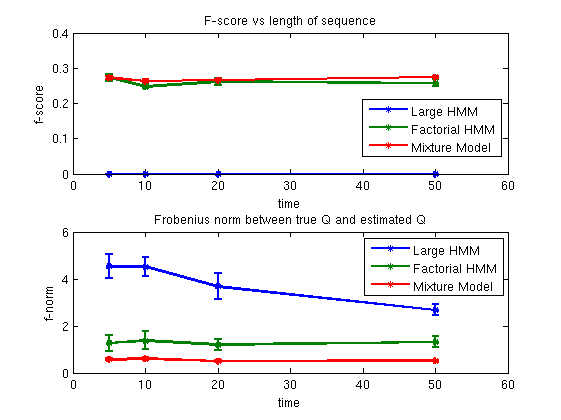
\includegraphics[scale=0.6]{results/mm_tvar}
  \caption{(a) F-score for the estimated weight evolution vs the true
    weight evolution sequence with increasing length of sequence, $T$. (b) Frobenius norm of the difference between the true
    evolution characteristics for the system and the estimated characteristics. }
  \label{fig:validation-t}
\end{figure}

\begin{figure}[h]
  \centering
  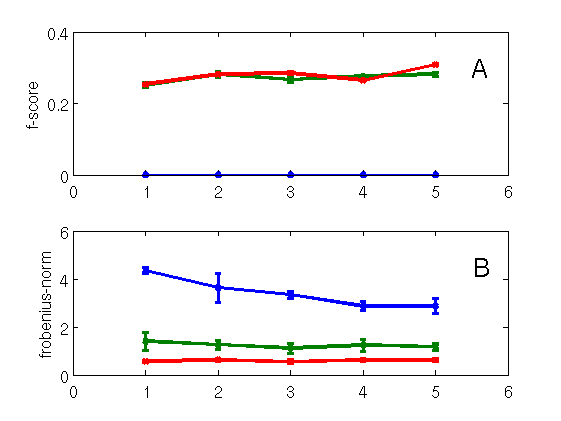
\includegraphics[scale=0.6]{results/mm_strain}
  \caption{(a) F-score for the estimated weight evolution vs the true
    weight evolution sequence with increasing number of strains. (b)
    Frobenius norm of the difference between the true evolution
    characteristics for the system and the estimated characteristics. } 
  \label{fig:validation-s}
\end{figure}


\subsection{Synthetic dataset}
\label{sec:synthetic-dataset}
% We consider a stochastic process $X(t) = \{x^1(t), \ldots, x^n(t)\}$
We generate a ``random'' graph $G=(V, E)$ with $C$ major components,
$\{A_1,\ldots, A_C\}$ with input parameters $p_{i}$ and $p_{c}$,
where $p_{i}$ is the probability, of an edge between two vertices in
the same component,  and $p_c$ is the probability of an edge between
two vertices in different components.  
%Each component has a transition probability matrix, $Q_c$, such that 

The activation level, $w_e(t)$ defined on an edge, $e$, belonging to
component, $A_k$, is a markov chain with transition probability matrix
$Q_{k}$. The problem is the estimation of the unknown transition probability
matrices $Q_k$ for each component, $A_k$. 

We use a noisy dirichlet prior for the estimation as follows: 
\begin{equation}
  \label{eq:exp1_prior}
\Theta^{(k)}  = Q_{k} + {\mathcal N}(0, \sigma^{2} I)   
\end{equation}
The experiment is conducted for $20$ trials with a graph of size
$N=50$ and number of components, $C$ chosen randomly between $2$ and
$10$. Figure~\ref{fig:exp1_fig} shows the F-scores for the
experiments done with multiple number of strains. 
% Figures~\ref{fig:exp1_fig} (b) shows the F-scores for the
% experiments with 2 strains with increasing number of missing gene.
 \begin{figure}[h]
   \centering
     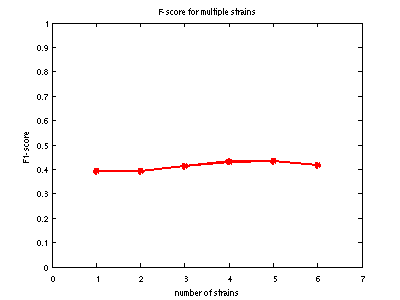
\includegraphics[scale=0.75]{results/Fig1_2}
%     & 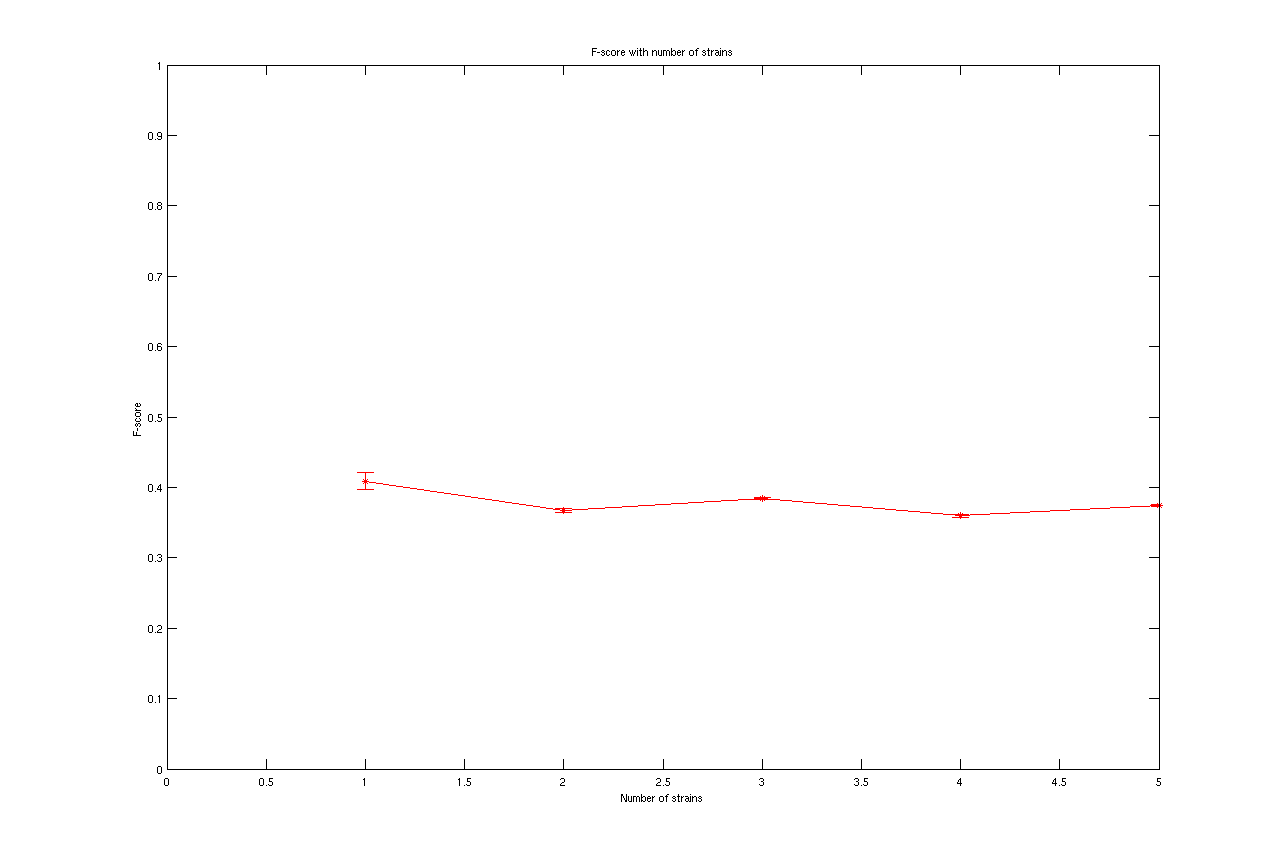
\includegraphics[scale=0.25]{results/f_score} \\
%     (a) & (b) 
%   \end{tabular}
   \caption{F-score for the synthetic dataset for multiple strains. We
     observe that increase in the number of strains provides more
     information about the activation strengths in the original
     network, which is visible in the slight increase in the
     F1-scores. However, since genes are being knocked out in each of
     the strains, the resulting is not equivalent to i.i.d. samples.  
   }
   \label{fig:exp1_fig}
 \end{figure}
% %We compare the performance of the factorial model and the mixture
% model against the standard HMM formulation\footnote{We use Kevin
%   Murphy's HMMall toolbox} %\href{http://people.cs.ubc.ca/~murphyk/Software/HMM/hmm.html}}

% Figure~\ref{fig:hmm} shows the results by employing the factorial
% assumption compared against the results obtained using the standard
% HMM.

 
% \subsection{}
%\subsection{Known networks}
%We take several networks consisting of genes  that are known to
%participate in the 

\section{Conclusion}
% \bibliographystyle{bioinformatics}
\bibliographystyle{plain}
\bibliography{default}
\appendix
% \section{Appendix}
% \subsection{Edge HMM}
% This section presents the derivation for the forward backward
% algorithm~\cite{Rabiner89hmm} under the factorial assumption for weights. 
% % We need to compute ${\mathcal L}(Q_{e};
% % Q_{e}^{n})$ in (\ref{eq:q-edge_em_map}), independently for each edge,
% % $e=(i,j)\in E$. This requires computing the conditional probability,
% % $P(\mathbf{w}_{e}^{1:T}| \mathbf{x}_{e}^{1:T}, Q_{e}^{(n)})$. 
% % We now outline the standard technique for parameter estimation in the
% % HMM~\cite{Rabiner89hmm} for the edge transition probabilities. 
%  The forward and the backward variables are defined as:
% \begin{eqnarray}
%   \label{eq:fwd}
%   f^{t}_{e}(l) &=& P(x_{e}^{1:S}(1:t) , w_{e}(t) = w_{l} | Q^{(n)}_{e}) \\
%   b^{t}_{e}(l) &=& P(x^{1:S}_{e}((t+1):T) | w_{e}(t) = w_{l}, Q^{(n)}_{e}) 
% \end{eqnarray}
% We assume that the data for strain, $s$, is independently generated based on the
% Ising model in (\ref{eq:ising}) with the weights that are damped
% versions (\ref{eq:edge-damping}) of the weights in the original
% strain. This leads to the observation model specified as:
% \begin{eqnarray}
%   \label{eq:obs}
%   o^{t}_{e}(l) &=& P(x_{e}^{1:S}(t) | w_{e}(t) = w_{l}) \\
% & = & \frac{1}{Z} \prod_{s=1}^{S} P(x_{e}^{s}(t) | w_{e}(t) = w_{l}) \\
% & = & \frac{\exp\left\{ - w_{l}\big(\sum_{s=1}^{S}
%       x^{s}_{i}(t)x^{s}_{j}(t) \Gamma^{s}(i,j)\big)
%   \right\}}{\sum^{\mathcal W}_{l=1}\exp\left\{ - w_{l}\big(\sum_{s=1}^{S}  x^{s}_{i}(t)x^{s}_{j}(t) \Gamma^{s}(i,j)\big) \right\}}
% \end{eqnarray}
% The update equations for computing the forward and backward variables
% are given as:
% \begin{eqnarray}
%   \label{eq:update}
%   f^{t+1}_{e}(m) &=& P(x_{e}^{1:S}(1:t) , w_{e}(t) = w_{l} | Q^{(n)}_{e}) \\
% o^{t+1}_{e}(m) \sum_{l=1}^{{\mathcal W}} f_{e}^{t}(l) q_{e}^{(n)}(l, m) \\
%   b^{t}_{e}(l) &=& P(x^{1:S}_{e}((t+1):T) | w_{e}(t) = w_{l}, Q^{(n)}_{e}) 
% \sum_{m=1}^{{\mathcal W}} q_{e}^{(n)}(l, m) o^{t+1}_{e}(m) b^{t+1}_{e}(m)
% \end{eqnarray}
% and the joint probability, $\xi_{e}^{t}(l,m)=P(w_{e}(t) =
% w_{l}, w_{e}(t+1) = w_{m} | x^{1:S}_{e}(1:T), Q^{(n)}_{e})$, is given as follows:
% \begin{eqnarray}
%   \label{eq:p-joint}
%   \xi_{e}^{t}(l,m) &=& \frac{f_{e}^{t}(l) q_{e}^{(n)}(l, m)
%     o_{e}^{t+1}(m) b^{t+1}(m)}{P(x^{1:S}(1:T) | Q^{(n)}_{e})} \\
% &=& \frac{f_{e}^{t}(l) q_{e}^{(n)}(l, m)
%     o_{e}^{t+1}(m) b^{t+1}(m)}{
%     \sum_{l, m} f_{e}^{t}(l) q_{e}^{(n)}(l, m)
%     o_{e}^{t+1}(m) b^{t+1}(m) }
% \end{eqnarray}
\end{document}